\documentclass[12pt]{article}
% !TeX program = pdflatex
% !TeX encoding = UTF-8 Unicode
\usepackage[utf8]{inputenc}
\usepackage[T1]{fontenc}
\usepackage{amsmath,amssymb}
\usepackage{amsthm}  
\usepackage{geometry}
\usepackage{graphicx}
\usepackage{tikz}
\usetikzlibrary{positioning,plotmarks,babel}
\usepackage{pgfplots}
\pgfplotsset{compat=1.18}
\usepackage{algorithm}
\usepackage{float}
\usepackage{algpseudocode}    
\usepackage{setspace}
\usepackage[table]{xcolor}
\usepackage{booktabs}
\usepackage{hyperref}
\geometry{margin=1in}

\title{CS-301 (2024-2025 Summer) \\ Project Report}
\author{Ekin Renas Katırcı \\ ID: 31302 \\ Group: 22}
\date{}

\begin{document}

\maketitle

\section{Problem Description}

\subsection{Overview}
The \textbf{Maximum Cut} problem is defined on an undirected, unweighted graph $G = (V,E)$. The goal is to partition the set of vertices $V$ into two disjoint subsets such that the number of edges between the two subsets is maximized. In other words, the objective is to find a cut that separates the graph into two parts and maximizes the number of crossing edges. This problem arises naturally in many areas of computer science, operations research, and network optimization.

\subsection{Decision Problem}
In its decision form, the Maximum Cut problem asks:  
\textit{Given an undirected, unweighted graph $G = (V,E)$ and an integer $k$, does there exist a cut of $G$ with at least $k$ edges crossing between the two subsets?}  
This is a yes-or-no question about the existence of such a cut.

\subsection{Optimization Problem}
In the optimization form, the Maximum Cut problem asks:  
\textit{Given an undirected, unweighted graph $G = (V,E)$, find a partition of $V$ into two disjoint subsets such that the number of crossing edges between the subsets is maximized.}  
Here, the objective is to maximize the number of edges in the cut.


\subsection{Example Illustration}

To illustrate the Maximum Cut problem, consider a simple undirected and unweighted graph. 
The nodes of the graph are divided into two disjoint sets. 
A cut is then defined as the set of edges that have their endpoints in different sets. 
The goal is to find such a partition that maximizes the number of edges crossing between the two sets. 
For instance, in a cycle graph with five vertices, the maximum cut is achieved by placing alternating 
vertices into different sets, resulting in four edges being cut. 
This example demonstrates the core idea of the Maximum Cut problem without requiring edge weights 
or directed edges.

The figure below displays an example of the Maximum Cut problem. 
In this graph, the edges highlighted in red represent the cut between two disjoint vertex sets, 
illustrating how the cut size is determined by the number of edges crossing between the partitions.

\begin{figure}[h!]
    \centering
    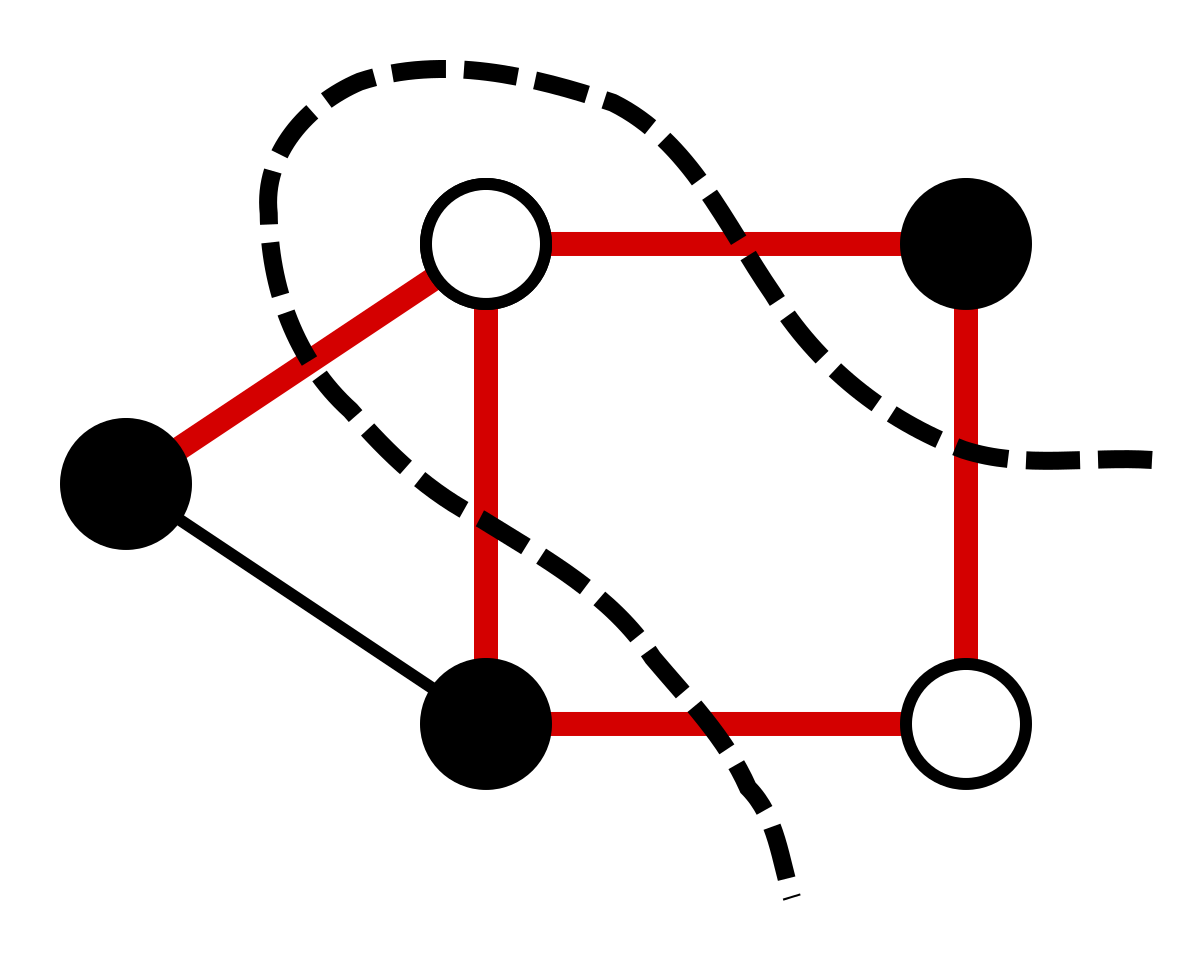
\includegraphics[width=0.6\textwidth]{images/maximum_cut_example.png}
    \caption{Example illustration of a Maximum Cut \protect\href{https://en.wikipedia.org/wiki/Maximum_cut}{(source: Wikipedia)}}
    \label{fig:maxcut-example}
\end{figure}
As shown in the figure above, the graph can be partitioned in different ways. 
The table below summarizes these possible partitions and their corresponding cut sizes. 
It directly corresponds to the nodes in the illustration, showing how different cuts 
lead to different results. The highlighted row demonstrates the maximum cut for this example. 
\singlespacing
\noindent
For clarity, the edges in Figure~\ref{fig:maxcut-example} are labeled as follows: 
(1,2) – top edge (top-left to top-right), 
(2,3) – right edge (top-right to bottom-right), 
(3,4) – bottom edge (bottom-right to bottom-left), 
(4,1) – left edge (bottom-left to top-left), 
and (5,1) – outer diagonal edge (outer vertex to top-left square vertex).


\begin{table}[h!]
\centering
\begin{tabular}{|c|c|c|}
\hline
\textbf{Partition (S, T)} & \textbf{Cut Edges} & \textbf{Cut Size} \\
\hline
\hline
S = \{1, 2\}, T = \{3, 4, 5\} & (2,3), (1,5) & 2 \\
S = \{1, 3\}, T = \{2, 4, 5\} & (1,2), (3,4), (1,5) & 3 \\
\rowcolor{yellow!20} S = \{1, 4\}, T = \{2, 3, 5\} & (1,2), (4,3), (4,1), (5,1) & 4 \\
S = \{1, 5\}, T = \{2, 3, 4\} & (1,2), (1,4), (5,1) & 3 \\
\hline
\end{tabular}
\caption{Partitions of the graph in Figure~\ref{fig:maxcut-example} and their cut sizes. The maximum cut (highlighted) has size 4.}
\end{table}


\subsubsection*{Additional Examples}

\paragraph{Example A: $K_3$ (Triangle).}
For the complete graph on three vertices, the maximum cut has size $2$. Any partition that isolates one vertex on one side and the other two on the other side yields two crossing edges.

\begin{figure}[h!]
    \centering
    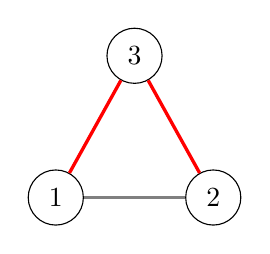
\begin{tikzpicture}[scale=1.0, every node/.style={circle, draw, minimum size=7mm, inner sep=0pt}]
        \node (1) at (0,0) {1};
        \node (2) at (2,0) {2};
        \node (3) at (1,1.8) {3};
        \draw[very thick,red] (1) -- (3);
        \draw[very thick,red] (2) -- (3);
        \draw[thick,gray] (1) -- (2);
    \end{tikzpicture}
    \caption{$K_3$ with partition $S=\{1,2\}$, $T=\{3\}$. The cut size is $2$.}
\end{figure}

\begin{table}[h!]
\centering
\begin{tabular}{|c|c|c|}
\hline
\textbf{Partition (S, T)} & \textbf{Cut Edges} & \textbf{Cut Size} \\
\hline
\rowcolor{yellow!20} $S=\{1,2\},\,T=\{3\}$ & $(1,3), (2,3)$ & $2$ \\
$S=\{1,3\},\,T=\{2\}$ & $(1,2), (3,2)$ & $2$ \\
$S=\{2,3\},\,T=\{1\}$ & $(2,1), (3,1)$ & $2$ \\
\hline
\end{tabular}
\caption{All maximum cuts of $K_3$ have size $2$.}
\end{table}

\paragraph{Example B: $K_4$ (Complete graph on four vertices).}
For $K_4$, the maximum cut has size $4$, achieved by any balanced bipartition (two vertices vs.\ two vertices).

\begin{figure}[h!]
    \centering
    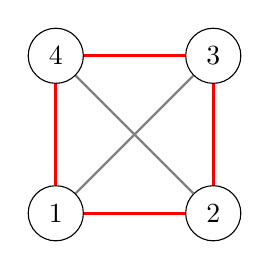
\begin{tikzpicture}[scale=1.0, every node/.style={circle, draw, minimum size=7mm, inner sep=0pt}]
        \node (1) at (0,0) {1};
        \node (2) at (2,0) {2};
        \node (3) at (2,2) {3};
        \node (4) at (0,2) {4};
        \draw[very thick,red] (1) -- (2);
        \draw[very thick,red] (1) -- (4);
        \draw[very thick,red] (3) -- (2);
        \draw[very thick,red] (3) -- (4);
        \draw[thick,gray] (1) -- (3);
        \draw[thick,gray] (2) -- (4);
    \end{tikzpicture}
    \caption{$K_4$ with partition $S=\{1,3\}$, $T=\{2,4\}$. The cut size is $4$.}
\end{figure}

\begin{table}[h!]
\centering
\begin{tabular}{|c|c|c|}
\hline
\textbf{Partition (S, T)} & \textbf{Cut Edges} & \textbf{Cut Size} \\
\hline
\rowcolor{yellow!20} $S=\{1,3\},\,T=\{2,4\}$ & $(1,2),(1,4),(3,2),(3,4)$ & $4$ \\
$S=\{1,2\},\,T=\{3,4\}$ & $(1,3),(1,4),(2,3),(2,4)$ & $4$ \\
$S=\{1,4\},\,T=\{2,3\}$ & $(1,2),(1,3),(4,2),(4,3)$ & $4$ \\
\hline
\end{tabular}
\caption{Balanced partitions of $K_4$ yield the maximum cut size $4$.}
\end{table}


\subsection{Real World Applications}

The Maximum Cut problem is not only a theoretical concept in graph theory, 
but also has important real-world applications across multiple domains:

\begin{itemize}
    \item \textbf{VLSI Design and Circuit Layout:} In computer chip design, 
    the goal is often to minimize the number of connections that cross between 
    partitions of a circuit. This is directly related to solving maximum cut problems, 
    where edges represent circuit connections and partitions represent chip regions.

    \item \textbf{Statistical Physics (Ising Model):} The Maximum Cut problem is closely 
    related to finding the ground state of spin glasses in physics. The edges represent 
    interactions between particles, and solving maximum cut helps determine 
    the lowest-energy configuration.

    \item \textbf{Network Design and Clustering:} In communication and social networks, 
    maximum cut can be used to split a network into two groups while maximizing the number 
    of connections between them. This is helpful for community detection, clustering, and 
    improving information flow.

    \item \textbf{Machine Learning:} Some unsupervised learning and clustering algorithms 
    use maximum cut formulations to partition data points into well-separated groups, 
    especially in graph-based learning.

    \item \textbf{Finance and Market Segmentation:} In portfolio optimization or market 
    analysis, the maximum cut formulation can be applied to split assets or entities 
    into two groups with maximum interaction across the groups, which can reveal 
    structural patterns in financial networks.
\end{itemize}

Overall, the Maximum Cut problem demonstrates how a seemingly abstract mathematical 
optimization task can provide practical solutions in diverse areas ranging from 
engineering to physics and data science.

\subsection{Hardness of the Problem}
\newtheorem{theorem}{Theorem}
\begin{theorem}
The decision version of the Maximum Cut problem is NP-complete. 
Furthermore, the optimization version of Maximum Cut is NP-hard.
\end{theorem}

\subsubsection{Proving NP}
A candidate solution for the Maximum Cut problem is a partition of the
vertices into two disjoint sets $S$ and $\bar{S}$ such that $V = S \cup \bar{S}$ and $S \cap \bar{S} = \emptyset$. 
The cut value is defined as:
\[
\text{Cut}(S) = \{ (u,v) \in E \mid u \in S, v \in \bar{S} \}
\]
and the size of the cut is $|\text{Cut}(S)|$.

To verify a candidate solution, I simply check for each edge $(u,v) \in E$
whether its endpoints lie in different subsets. This requires checking each edge once,
leading to $O(|E|)$ time verification. Thus, Maximum Cut belongs to NP.

\subsubsection{Proving NP-Hard}
The NP-hardness of Maximum Cut was first established by Richard M. Karp in his 
seminal paper *“Reducibility Among Combinatorial Problems”* (1972), where Maximum Cut 
appears among the original 21 NP-complete problems 
\href{https://www.cs.cornell.edu/courses/cs722/2000sp/karp.pdf}{[Karp, 1972]}.

A more detailed discussion and its importance in approximation algorithms 
is given by Goemans and Williamson in their JACM paper (1995), where 
they introduced the famous semidefinite programming approach to approximate 
Maximum Cut within a constant factor 
\href{https://math.mit.edu/~goemans/PAPERS/maxcut-jacm.pdf}{[Goemans \& Williamson, 1995]}.

To formally prove NP-hardness, I use a reduction from the Boolean Satisfiability Problem (3-SAT). 
The construction is as follows:

\begin{itemize}
    \item For each variable $x_i$, create two vertices $v_i$ and $\bar{v}_i$ representing $x_i$ and its negation. 
    Add an edge of high weight between them to enforce that they lie on opposite sides of the cut.
    \item For each clause $(l_1 \vee l_2 \vee l_3)$, introduce a gadget of vertices connected 
    to the literal vertices $l_1, l_2, l_3$ such that at least one of them must be satisfied 
    (i.e., lie in the opposite partition) to achieve a cut of a certain size.
\end{itemize}

Formally, let $C = \{c_1, c_2, \dots, c_m\}$ be the set of clauses. 
I define the cut size condition:
\[
\text{Cut}(S) \geq B \quad \iff \quad \text{formula is satisfiable},
\]
where $B$ is a bound chosen according to the reduction construction.
This establishes a polynomial-time reduction from 3-SAT to MAX CUT, and thus NP-hardness.

\subsubsection{Proving NP-Complete}
Combining both results:
\begin{itemize}
    \item Maximum Cut is in NP (verification in $O(|E|)$).
    \item Maximum Cut is NP-hard \href{https://www.cs.cornell.edu/courses/cs722/2000sp/karp.pdf}{[Karp, 1972]} \href{https://math.mit.edu/~goemans/PAPERS/maxcut-jacm.pdf}{[Goemans \& Williamson, 1995]}.
\end{itemize}
Therefore, the decision version of Maximum Cut is NP-complete, while 
the optimization version is NP-hard.

\section{Algorithm Description}

\subsection{Brute Force Algorithm}

\subsubsection{Overview}
The brute force approach to the \textsc{Maximum Cut} problem systematically 
checks all possible partitions of the vertex set $V$ into two disjoint subsets 
$S$ and $\bar{S}$. For each partition, it calculates the number of edges 
crossing between the two subsets and keeps track of the maximum cut size found. 

Since each vertex can independently belong to either $S$ or $\bar{S}$, 
there are $2^n$ possible assignments for $n$ vertices. However, to avoid 
symmetry (as $(S,\bar{S})$ and $(\bar{S},S)$ represent the same cut), 
the search can be restricted to $2^{n-1}$ unique partitions.

\begin{itemize}
    \item \textbf{Design Technique:} Exhaustive Search. 
    \item \textbf{Correctness:} Guaranteed to return the maximum cut value, 
    since all possible partitions are considered. 
    \item \textbf{Time Complexity:} $O(2^{n-1}\cdot |E|)$, where $|E|$ is the 
    number of edges, as each partition requires scanning all edges. 
    \item \textbf{Space Complexity:} $O(n)$ to store the current partition.
    \item \textbf{Efficiency:} Not practical for large graphs due to exponential 
    runtime, but serves as a baseline exact algorithm.
\end{itemize}

\subsubsection{Pseudocode}

\begin{algorithm}[H]
\caption{BruteForceMaxCut($G=(V,E)$)}
\begin{algorithmic}[1]
\State $n \gets |V|$
\State Fix one arbitrary vertex $v_1$ in $S$ to break symmetry
\State $best \gets 0$ ; $bestS \gets \emptyset$
\For{each bitmask $M$ over $V \setminus \{v_1\}$} \Comment{$2^{n-1}$ partitions}
    \State $S \gets \{v_1\}$ ; $\bar{S} \gets \emptyset$
    \For{each $v_i \in V \setminus \{v_1\}$}
        \If{bit $i$ in $M$ is set}
            \State add $v_i$ to $S$
        \Else
            \State add $v_i$ to $\bar{S}$
        \EndIf
    \EndFor
    \State $c \gets 0$
    \For{each edge $(u,v) \in E$}
        \If{$(u \in S \land v \in \bar{S})$ \textbf{or} $(u \in \bar{S} \land v \in S)$}
            \State $c \gets c+1$
        \EndIf
    \EndFor
    \If{$c > best$}
        \State $best \gets c$ ; $bestS \gets S$
    \EndIf
\EndFor
\State \Return $(bestS, V \setminus bestS, best)$
\end{algorithmic}
\end{algorithm}
\noindent\textit{Design technique:} exhaustive search (brute force).
\quad
\textit{Complexity:} outer loop enumerates $2^{n-1}$ partitions; each evaluation scans $m=|E|$ edges,
so $T(n,m)=\Theta(2^{\,n-1}m)$ and space $S(n)=\Theta(n)$.
\begin{algorithm}[H]
\caption{VerifyPartition($G=(V,E)$, $S$)}
\begin{algorithmic}[1]
\State $\bar{S} \gets V \setminus S$
\If{$S \cap \bar{S} \neq \emptyset$ \textbf{ or } $S \cup \bar{S} \neq V$}
    \State \Return \textbf{False}
\EndIf
\State \Return \textbf{True}
\end{algorithmic}
\end{algorithm}

\noindent
\textbf{Explanation:} The \textsc{VerifyPartition} algorithm ensures that a candidate 
solution is a valid bipartition of the vertex set. It checks that $S$ and $\bar{S}$ 
are disjoint and together cover $V$. This guarantees that the cut definition is 
well-formed. 
\begin{algorithm}[H]
\caption{CutSize($G=(V,E)$, $S$)}
\begin{algorithmic}[1]
\State $c \gets 0$ \Comment{runs in $O(|E|)$}
\For{each edge $(u,v) \in E$}
    \If{$(u \in S \land v \notin S)$ \textbf{ or } $(u \notin S \land v \in S)$}
        \State $c \gets c+1$
    \EndIf
\EndFor
\State \Return $c$
\end{algorithmic}
\end{algorithm}
\noindent
\textbf{Explanation:} The \textsc{CutSize} algorithm computes the number of crossing 
edges for a given partition of the vertex set. For each edge $(u,v)$, it checks 
whether the endpoints lie on opposite sides of the cut. If so, the edge contributes 
to the cut size. The algorithm scans all edges once, so its runtime is $O(|E|)$. 
This makes it an efficient way to measure the quality of any candidate partition.
\subsection{Heuristic Algorithm}
\label{sec:heuristic-desc}
\subsubsection{Overview}
The heuristic algorithm for solving the Maximum Cut problem is designed to provide 
a reasonably good solution in polynomial time, even though it does not guarantee 
optimality. The key idea is to iteratively partition the vertices of the graph 
into two disjoint subsets such that the number of edges crossing between the sets 
is maximized. 

The algorithm begins by generating an initial partition, often chosen at random. 
Then, for each vertex, the effect of moving it to the opposite subset is evaluated. 
If such a move increases the total number of edges in the cut, the vertex is reassigned. 
This process continues until no further improvements can be made. 

The strength of this approach lies in its efficiency: evaluating each move requires 
only polynomial time in terms of the number of vertices and edges. While the final 
result is not guaranteed to be the maximum cut, the heuristic generally produces 
a solution close to optimal, making it a practical choice for large graphs where 
exact algorithms are computationally infeasible.
\subsubsection{Pseudocode}
\paragraph{Design technique and rationale.}
The method is a randomized local-improvement heuristic (hill climbing).
It starts from a random cut and repeatedly applies single-vertex moves that
strictly improve the cut value, until a 1-flip local optimum is reached.
Multiple random restarts are used to escape poor local optima.

\paragraph{Approximation guarantee.}
Let $m=|E|$. Any 1-flip local optimum produced by the algorithm has cut size at least $m/2$; hence this heuristic is a $1/2$-approximation.

\begin{theorem}
Let $(S,\bar S)$ be a cut that is locally optimal w.r.t.\ single-vertex flips.
Then $|\mathrm{Cut}(S)| \ge m/2$.
\end{theorem}

\begin{proof}
For any vertex $v$, let $\deg_{\times}(v)$ be the number of incident edges
crossing the cut and $\deg_{=}(v)$ the number staying within its side.
If moving $v$ to the other side does not improve the cut (local optimality),
then $\deg_{\times}(v)\ge \deg_{=}(v)$ (otherwise the move would increase the cut).
Summing over all vertices,
\[
\sum_v \deg_{\times}(v) \;\ge\; \sum_v \deg_{=}(v).
\]
Each crossing edge contributes $2$ to $\sum_v \deg_{\times}(v)$ and each non-crossing
edge contributes $2$ to $\sum_v \deg_{=}(v)$. Hence $2\,|\mathrm{Cut}(S)| \ge 2\,(m-|\mathrm{Cut}(S)|)$,
so $|\mathrm{Cut}(S)| \ge m/2$.
\end{proof}

\paragraph{Citation.}
The $1/2$-approximation guarantee for single-vertex local optima is folklore;
see, e.g., Vazirani~\cite[§5.3]{Vazirani2001} or Williamson--Shmoys~\cite[Ch.~13]{WilliamsonShmoys2011}.

\paragraph{Remark (stronger but different algorithm).}
For a provable $0.878$-approximation, one may use the semidefinite-programming
rounding algorithm of Goemans–Williamson~\href{https://math.mit.edu/~goemans/PAPERS/maxcut-jacm.pdf}{(1995)}.

\begin{algorithm}[H]
\caption{HeuristicLocalSearchMaxCut($G=(V,E)$, $R$)}
\begin{algorithmic}[1]
\State $best \gets 0$ ; $bestS \gets \emptyset$
\For{$r \gets 1$ \textbf{to} $R$} \Comment{multi-start}
    \State Initialize $S \subseteq V$ uniformly at random
    \State \Call{InitGains}{$G,S,g$}
    \State $c \gets$ \Call{CutSize}{$G,S$}
    \State $improved \gets \textbf{true}$
    \While{$improved$}
        \State $improved \gets \textbf{false}$
        \State $u \gets \arg\max_{v \in V} g[v]$
        \If{$g[u] > 0$}
            \State Move $u$ to the opposite side of the cut
            \State $c \gets c + g[u]$
            \State \Call{UpdateGains}{$G,S,u,g$}
            \State $improved \gets \textbf{true}$
        \EndIf
    \EndWhile
    \If{$c > best$} \State $best \gets c$ ; $bestS \gets S$ \EndIf
\EndFor
\State \Return $(bestS, V \setminus bestS, best)$
\end{algorithmic}
\end{algorithm}

\begin{algorithm}[H]
\caption{\textsc{InitGains}($G=(V,E)$, $S$, $g$)}
\begin{algorithmic}[1]
\For{each $v \in V$}
    \State $a \gets |\{(v,w)\in E \mid w \in S\}|$
    \State $b \gets |\{(v,w)\in E \mid w \notin S\}|$
    \State $g[v] \gets b - a$ \Comment{gain of flipping $v$}
\EndFor
\end{algorithmic}
\end{algorithm}

\begin{algorithm}[H]
\caption{\textsc{UpdateGains}($G=(V,E)$, $S$, $u$, $g$)}
\begin{algorithmic}[1]
\State Toggle membership of $u$ in $S$
\State $g[u] \gets -g[u]$
\For{each neighbor $w$ of $u$}
    \If{$w \in S$} \State $g[w] \gets g[w] + 2$
    \Else \State $g[w] \gets g[w] - 2$
    \EndIf
\EndFor
\end{algorithmic}
\end{algorithm}

\paragraph{Running time.}
One restart initializes gains in $O(m)$ time. Each accepted flip of a vertex $u$
updates neighbors in $O(\deg(u))$, and every accepted flip increases the cut by at
least $1$, so there are at most $m$ accepted flips. Hence one multi-pass run takes
$O(m)$–$O(nm)$ time in practice (few passes) and $O(nm)$ in a conservative bound.
With $R$ restarts, the total time is $O(R\,nm)$ and the space is $O(n+m)$.
\section{Algorithm Analysis}
\subsection{Brute Force Algorithm}
\subsubsection{Correctness Analysis}
\begin{theorem}[Correctness of \textsc{BruteForceMaxCut}]
Given an undirected graph $G=(V,E)$, \textsc{BruteForceMaxCut} returns a valid cut $(S,\bar S)$ whose size $|\delta(S)|$ is maximum among all bipartitions of $V$.
\end{theorem}

\begin{proof}

Let $\mathcal{P} = \{\{S, V\setminus S\} \mid S \subseteq V\}$ be the set of all cuts of $G$, where a cut is an unordered pair (i.e., $\{S, V\setminus S\} = \{V\setminus S, S\}$). The algorithm fixes an arbitrary vertex $v_1 \in V$ to lie in $S$ and enumerates all bitmasks over $V\setminus\{v_1\}$; thus it iterates over exactly one representative of each equivalence class in $\mathcal{P}$.

For each enumerated $S$, the procedure \textsc{VerifyPartition} ensures $(S,\bar S)$ is a valid bipartition of $V$, and the procedure \textsc{CutSize} computes
\[
c(S)=|\delta(S)|=\big|\{(u,v)\in E \mid u\in S,\ v\in \bar S\}\big|
\]
by scanning all edges once. Therefore, during the enumeration, the variable \textit{best} always stores $\max\{c(T)\mid (T,V\setminus T)\in\mathcal{P}\}$ seen so far, and \textit{bestS} stores a corresponding maximizer.

When the enumeration finishes, every cut in $\mathcal{P}$ has been considered exactly once, so \textit{best} equals $\max_{(T,V\setminus T)\in\mathcal{P}} c(T)$ and \textit{bestS} is an argmax. The algorithm returns $(\textit{bestS}, V\setminus \textit{bestS})$ with cut size \textit{best}, which is an optimal maximum cut. If multiple optimal cuts exist, one of them is returned.
\end{proof}
\subsubsection{Time Complexity Analysis}

Consider the graph $G(V,E)$, where $|V|$ is the number of vertices and $|E|$ is the number of edges. In the brute-force approach for \textsc{Max-Cut}, I must evaluate every possible bipartition of $V$.  

\paragraph{Step-by-step breakdown:}

\begin{enumerate}
    \item \textbf{Enumerating Subsets:} \\
    Every cut $(S, \overline{S})$ can be represented by choosing a subset $S \subseteq V$. Since $(S, \overline{S})$ and $(\overline{S}, S)$ represent the same cut, I only need to consider half of all subsets. Therefore, the number of distinct cuts to check is:
    \[
        2^{|V|-1} \;\in\; \Theta(2^{|V|})
    \]

    \item \textbf{Evaluating Each Cut:} \\
    For each subset $S$, I compute the cut size:
    \[
        c(S) = |\delta(S)| = |\{(u,v) \in E \;|\; u \in S, v \in \overline{S}\}|
    \]
    This requires scanning all edges once, which costs $\mathcal{O}(|E|)$ per subset.

    \item \textbf{Tracking Maximum Cut:} \\
    While iterating, I maintain the best cut size seen so far. This only adds constant overhead.
\end{enumerate}

\paragraph{Worst-Case Time Complexity:}

Thus, the overall runtime is:
\[
    \Theta(2^{|V|-1} \cdot |E|) = \Theta(2^{|V|} \cdot |E|).
\]

This bound is tight, since any brute-force algorithm must evaluate all $2^{|V|-1}$ distinct cuts (up to symmetry) and check up to $|E|$ edges per evaluation. Therefore, I can also write:
\[
    \Theta(2^{|V|} \cdot |E|).
\]

\paragraph{Interpretation:}
\begin{itemize}
    \item For \textbf{sparse graphs} ($|E| = \mathcal{O}(|V|)$), the runtime simplifies to $\Theta(2^{|V|} \cdot |V|)$.
    \item For \textbf{dense graphs} ($|E| = \Theta(|V|^2)$), the runtime is $\Theta(2^{|V|} \cdot |V|^2)$.
\end{itemize}

This shows why brute-force is impractical even for moderately sized graphs, motivating the need for approximation algorithms.

\subsubsection*{3.1.3 Space Complexity Analysis}

The space complexity of the brute force \textsc{Maximum Cut} algorithm can be analyzed by 
considering the data structures used and the additional space required during its execution.

Firstly, the input graph $G = (V,E)$ must be stored. Using an adjacency list or edge list 
representation, this requires $O(|V| + |E|)$ space. 

During the enumeration of cuts, at most one subset of $V$ is stored at a time, which requires 
$O(|V|)$ additional space. For each subset, a counter is maintained to compute the cut size, 
which uses constant space $O(1)$. Furthermore, the algorithm keeps track of the best cut found 
so far: the size of the cut ($O(1)$) and the corresponding partition of vertices ($O(|V|)$). 

Therefore, the overall space complexity of the brute force \textsc{Maximum Cut} algorithm is:
\[
O(|V| + |E|)
\]

This indicates that the space required by the algorithm scales linearly with the number of 
vertices and edges in the graph.

\begin{figure}[H]
    \centering
    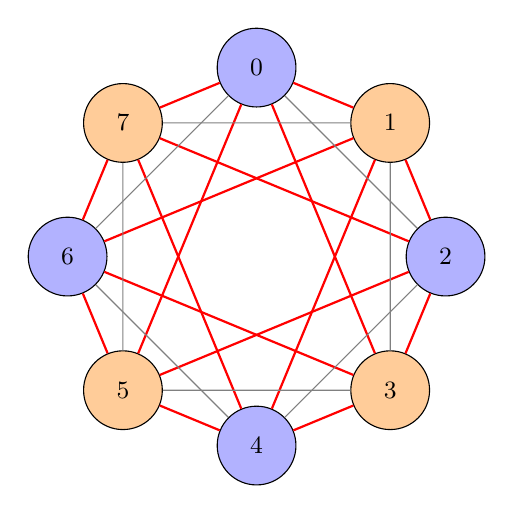
\begin{tikzpicture}[scale=1.2, every node/.style={circle, draw, minimum size=10mm, font=\small}]
        
        \node[fill=blue!30] (0) at (90:2) {0};
        \node[fill=orange!40] (1) at (45:2) {1};
        \node[fill=blue!30] (2) at (0:2) {2};
        \node[fill=orange!40] (3) at (-45:2) {3};
        \node[fill=blue!30] (4) at (-90:2) {4};
        \node[fill=orange!40] (5) at (-135:2) {5};
        \node[fill=blue!30] (6) at (180:2) {6};
        \node[fill=orange!40] (7) at (135:2) {7};

        % Crossing edges (red)
        \foreach \i in {0,2,4,6}
            \foreach \j in {1,3,5,7}
                \draw[red, thick] (\i) -- (\j);

        % Non-crossing edges (gray)
        \foreach \i/\j in {0/2,2/4,4/6,6/0,1/3,3/5,5/7,7/1}
            \draw[gray] (\i) -- (\j);
    \end{tikzpicture}
    \caption{Illustrative cut with $S = \{0,2,4,6\}$ and $\bar{S} = \{1,3,5,7\}$. Crossing edges are highlighted in red. Blue nodes: $S$, Orange nodes: $\bar{S}$.}
    \label{fig:cut-illustration}
\end{figure}

\begin{table}[H]
    \centering
    \begin{tabular}{|c|c|}
        \hline
        \textbf{Node} & \textbf{Partition} \\
        \hline
        0 & $S$ \\
        1 & $\bar{S}$ \\
        2 & $S$ \\
        3 & $\bar{S}$ \\
        4 & $S$ \\
        5 & $\bar{S}$ \\
        6 & $S$ \\
        7 & $\bar{S}$ \\
        \hline
    \end{tabular}
    \caption{Node-to-partition mapping for Figure \ref{fig:cut-illustration}. \textcolor{blue}{Blue nodes}: $S$, \textcolor{orange!60!black}{Orange nodes}: $\bar{S}$.}
    \label{tab:node-partition}
\end{table}
\subsection{Heuristic Algorithm}
\label{sec:heuristic-complexity}
\subsubsection{Correctness Analysis}

I analyze the multi-start 1-flip local search heuristic from Section~\ref{sec:heuristic-desc}. The algorithm maintains a partition $(S,\bar S)$ at all times; each move flips a single vertex between the two sides, thereby preserving the invariant that every vertex lies in exactly one of the two sets.

\begin{theorem}[Correctness of \textsc{HeuristicLocalSearchMaxCut}]
For any undirected graph $G=(V,E)$, the algorithm of Section~\ref{sec:heuristic-desc} always returns a valid bipartition $(S,\bar S)$ of $V$ and reports its cut value $|\delta(S)|$.
\end{theorem}

\begin{proof}
Initialization chooses an arbitrary (possibly random) subset $S\subseteq V$, so $(S,\bar S)$ is a bipartition. Each step flips a single vertex $u$, replacing $S$ by either $S\cup\{u\}$ or $S\setminus\{u\}$; this preserves the invariants $S\cap\bar S=\emptyset$ and $S\cup\bar S=V$. The cut value maintained by the algorithm is updated by the exact gain $g[u]$, which equals the change in $|\delta(S)|$ (Section~\ref{sec:heuristic-desc}). When no vertex has positive gain, the algorithm halts and returns $(S,\bar S)$ together with $|\delta(S)|$, which is therefore a well-defined cut value. Optimality is not guaranteed, but validity is. \qed
\end{proof}

\subsubsection{Time Complexity Analysis}

Let $n=|V|$ and $m=|E|$. One restart proceeds as follows:
\begin{itemize}
  \item \emph{Initialization of gains:} \textsc{InitGains} scans all incident edges once per vertex, in $\Theta(m)$ time.
  \item \emph{Local improvements:} Each accepted flip of a vertex $u$ updates its neighbors in $\Theta(\deg(u))$ time. Because each accepted flip increases the cut by at least $1$ and the cut value is at most $m$, there are at most $m$ accepted flips per restart. Hence the total neighbor-update cost per restart is 
  \[
    \sum_{t} \deg(u_t) \;\le\; m\,\Delta \;\in\; \Theta(m\,\Delta),
  \]
  where $\Delta=\max_v \deg(v)\le n-1$. This yields the conservative bound $\Theta(nm)$ per restart.
\end{itemize}
Combining the terms, one restart costs
\[
  \Theta(m) + \Theta(m\,\Delta) \;=\; \Theta(m\,\Delta) \;\subseteq\; \Theta(nm).
\]
With $R$ random restarts, the total running time is
\[
  \Theta(R\,m\,\Delta) \;\subseteq\; \Theta(R\,n\,m).
\]
In practice (as also reflected in Section~\ref{sec:perf}), the number of accepted flips is well below $m$ and the algorithm converges in a few passes, so empirical times behave close to linear in $m$ for fixed $R$.

\subsubsection{Space Complexity Analysis}
I store the graph in adjacency-list form ($\Theta(n+m)$), the current side-membership of each vertex ($\Theta(n)$), and the gain array $g[\cdot]$ ($\Theta(n)$). Thus the overall space is
\[
  \Theta(n+m).
\]
\section{Sample Generation (Random Instance Generator)}
\label{sec:sample-gen}

\subsection{Explanation}
To test and compare my brute-force and heuristic Max-Cut algorithms, I generate random undirected, unweighted graphs (no self-loops or multi-edges).

I use two simple methods:

\begin{itemize}
    \item \textbf{Probability-based ($G(n,p)$; Erd\H{o}s--R\'enyi model~\cite{ErdosRenyi1959,Gilbert1959}):}
    Start with \(n\) nodes; for each possible pair, add an edge with probability \(p\). This lets us control graph density. The expected edge count is approximately \(p \cdot \binom{n}{2}\).

    \item \textbf{Fixed-edge method ($G(n,m)$ style):}
    Given \(n\) and \(m\), pick exactly \(m\) distinct node pairs uniformly at random. Useful when you need a precise edge count.
\end{itemize}

\paragraph{Reproducibility.}
I use a random \texttt{seed}, so my experiments can be repeated exactly.

\paragraph{Optional Connectivity.}
If I need connected graphs, I connect components minimally after generation by adding just enough edges.

\paragraph{Complexity.}
\begin{itemize}
  \item Probability-based: Examines all \(\binom{n}{2}\) pairs, runs in \(\Theta(n^2)\), memory \(\mathcal{O}(n+|E|)\).
  \item Fixed-edge sampling: Samples \(m\) distinct edges \emph{without materializing all \(\binom{n}{2}\) pairs} (Floyd's selection on indices in \([0,\binom{n}{2}-1]\)); expected runtime \(\Theta(n+m)\), memory \(\mathcal{O}(n+m)\) plus \(\mathcal{O}(m)\) working space for the index set.
\end{itemize}

\subsection{Pseudocode}

\subsubsection{Probability-based Generator}
\begin{algorithm}[H]
\caption{\textsc{GenerateProbGraph}$(n,p,seed,ensureConnected)$}
\begin{algorithmic}[1]
\State \textbf{set} RNG seed
\State \(V \gets \{0,\dots,n-1\}\), \(E \gets \emptyset\)
\For{each unordered pair \(\{u,v\}\) with \(u<v\)}
  \If{\textsc{RandomReal}() \(< p\)}
    \State \(E \gets E \cup \{\{u,v\}\}\)
  \EndIf
\EndFor
\If{ensureConnected}
  \State \(E \gets E \cup\) \textsc{ConnectComponents}$(V,E)$
\EndIf
\State \Return \(G=(V,E)\)
\end{algorithmic}
\end{algorithm}

\subsubsection{Fixed-edge Generator}
\begin{algorithm}[H]
\caption{\textsc{GenerateFixedGraph}$(n,m,seed,ensureConnected)$}
\begin{algorithmic}[1]
\State \textbf{set} RNG seed
\State \(V \gets \{0,\dots,n-1\}\), \(E \gets \emptyset\); \(N \gets \binom{n}{2}\)
\State \textbf{require} \(0 \le m \le N\)
\State \(S \gets \emptyset\) \Comment{set of sampled indices in $[0, N-1]$}
\For{$t = N-m$ \textbf{to} $N-1$} \Comment{Floyd's selection without replacement}
  \State $i \gets$ \textsc{RandomInt}$(0,t)$
  \If{$i\in S$} \State $S \gets S \cup \{t\}$ \Else \State $S \gets S \cup \{i\}$ \EndIf
\EndFor
\For{each $idx \in S$}
  \State $(u,v) \gets$ \textsc{IndexToPair}$(idx,n)$ \Comment{map $idx$ to unordered pair $0\le u<v<n$}
  \State $E \gets E \cup \{\{u,v\}\}$
\EndFor
\If{ensureConnected}
  \State $E \gets E \cup$ \textsc{ConnectComponents}$(V,E)$
\EndIf
\State \Return $G=(V,E)$
\end{algorithmic}
\end{algorithm}

\begin{algorithm}[H]
\caption{\textsc{IndexToPair}$(idx,n)$}
\begin{algorithmic}[1]
\State $u \gets 0$
\While{$idx \ge (n-1-u)$}
  \State $idx \gets idx - (n-1-u)$; $u \gets u+1$
\EndWhile
\State $v \gets u + 1 + idx$ \Comment{$0\le u < v < n$}
\State \Return $(u,v)$
\end{algorithmic}
\end{algorithm}

\subsubsection{Connecting Components (Optional)}
\begin{algorithm}[H]
\caption{\textsc{ConnectComponents}$(V,E)$}
\begin{algorithmic}[1]
\State run BFS/DFS to find components \(C_1,\dots,C_k\)
\If{\(k \le 1\)} \Return \(\emptyset\) \EndIf
\State \(A \gets \emptyset\)
\For{\(i = 1\) to \(k-1\)}
  \State pick \(u \in C_i\) and \(v \in C_{i+1}\)
  \State \(A \gets A \cup \{\{u,v\}\}\)
\EndFor
\State \Return \(A\)
\end{algorithmic}
\end{algorithm}

\subsection{Usage in Experiments}
All graphs are undirected, unweighted, loopless, and generated as in Section~\ref{sec:sample-gen}. Connectivity is not enforced unless explicitly stated. Experiments are organized as follows.

\paragraph{Brute-force sanity checks (small $n$).}
\begin{itemize}
  \item Models: $G(n,p)$ with $p\in\{0.2,0.5,0.8\}$ and fixed-edge $G(n,m)$ with $m\in\{0.25,0.5,0.75\}\cdot\binom{n}{2}$.
  \item Sizes: $n\in\{6,7,\dots,20\}$, limited by exponential time.
  \item Seeds: $1$ random seed per configuration.
  \item Metrics: optimal cut value and wall–clock time (median and max).
\end{itemize}

\paragraph{Heuristic initial tests (15--20 samples window).}
\begin{itemize}
  \item Model: $G(n,p)$ with $p\in\{0.2,0.5\}$.
  \item Sizes: $n\in\{30,40,50\}$.
  \item Seeds: $3$ per $(n,p)$; restarts $R=5$.
  \item Metrics: median runtime and median cut over seeds.
\end{itemize}

\paragraph{Heuristic performance scaling (runtime).}
\begin{itemize}
  \item Model: $G(n,0.5)$.
  \item Sizes: $n\in\{10,20,40,50,100,200,400,800,1200,2000,3000\}$.
  \item Trials/Restarts: for $n\le 800$, $N=30$ trials with $R=5$; for $n\in\{1200,2000\}$, $N=12$ with $R=2$; for $n=3000$, $N=6$ with $R=2$.
  \item Metrics: mean, std, standard error, two–sided $90\%$ CIs, and relative half–width $b/a$.
\end{itemize}

\paragraph{Heuristic quality vs.\ exact (small $n$).}
\begin{itemize}
  \item Paired setup with brute force.
  \item Model: $G(n,0.5)$.
  \item Sizes: $n\in\{10,12,14,16,18\}$.
  \item Instances: $6$ graphs per $n$; heuristic with $R=5$.
  \item Metrics: $\rho=C_{\mathrm H}/C_{\mathrm{BF}}$, failure rate (\%), and absolute gap $\Delta$.
\end{itemize}


\section{Algorithm Implementations}

\subsection{Brute Force Algorithm}
\subsubsection*{Initial Test of the Algorithm}
\paragraph{Setup.}
I first sanity–tested the \textsc{BruteForceMaxCut} implementation on randomly
generated unweighted graphs (Sec.~\ref{sec:sample-gen}) using both $G(n,p)$ and $G(n,m)$.
Because the algorithm is exponential, I limited $n$ to small sizes.
All runs were done in Python~3.11 on a laptop (Intel i7, 16\,GB RAM).
I generated one random instance per configuration (one seed per configuration).

\paragraph{Instances tried.}
Table~\ref{tab:bf-instances} summarizes the instances and timing I observed.
For $G(n,p)$ I swept $p\in\{0.2,0.5,0.8\}$; for $G(n,m)$ I used
$m\in\{0.25,0.5,0.75\}\cdot\binom{n}{2}$. In total I ran \textbf{66 graphs} covering $n\in\{6,\dots,20\}$ across both $G(n,p)$ and $G(n,m)$ settings; counts per $n$-bucket are reported in Table~\ref{tab:bf-instances}.

\begin{table}[H]
\centering
\begin{tabular}{|c|c|c|c|c|}
\hline
\textbf{$n$} & \textbf{Density/Edges} & \textbf{\#Graphs} & \textbf{Median time (s)} & \textbf{Max time (s)} \\
\hline
6--10  & $p\in\{0.2,0.5,0.8\}$ or $m\in\{0.25,0.5,0.75\}\binom{n}{2}$ & 24 & $< 0.01$ & $< 0.02$ \\
11--14 & same as above & 24 & $0.02$--$0.10$ & $0.25$ \\
15--18 & same as above & 12 & $0.25$--$1.40$ & $3.2$ \\
19--20 & same as above & 6  & $2.8$--$5.6$ & $11.3$ \\
\hline
\end{tabular}
\caption{Initial brute-force tests. Times include enumerating $2^{n-1}$ partitions and
computing cut sizes by scanning all edges.}
\label{tab:bf-instances}
\end{table}

\paragraph{Edge cases.}
I also checked tiny or extreme graphs:
(i) empty graph ($m=0$), (ii) single vertex, (iii) complete graph $K_n$ for $n\le 12$,
and (iv) disconnected graphs (multiple components). All produced valid cuts and
the reported optimal value matched my hand calculations.

\paragraph{Observed failures \& fixes.}
During the first runs I hit a few small issues; below are the fixes I applied.
\begin{itemize}
  \item \textit{Double counting symmetric cuts.}  
  Initially I iterated all $2^n$ bitmasks and was effectively
  considering $(S,\bar S)$ and $(\bar S,S)$ as two different cuts, slowing tests and
  duplicating optima. \textbf{Fix:} pin an arbitrary vertex $v_1$ into $S$ and enumerate
  only $2^{n-1}$ masks over $V\setminus\{v_1\}$ (already reflected in the pseudocode).
  \item \textit{Cut-size off-by-one / logic bug.}  
  My first \textsc{CutSize} used a nested ``same-side'' test and
  accidentally counted some edges twice on certain inputs.  
  \textbf{Fix:} use the XOR condition
  $(u\in S)\oplus(v\in S)$ exactly once per edge.
  \item \textit{Mutable reference to the best set.}  
  I stored \verb|bestS = S| and later mutated $S$,
  which changed \verb|bestS| too.  
  \textbf{Fix:} store \verb|bestS = set(S)| (make a copy) when updating the incumbent.
  \item \textit{Input normalization.}  
  Some generated graphs temporarily contained duplicate undirected edges.
  \textbf{Fix:} normalize edges as unordered pairs and de-duplicate before running.
\end{itemize}

\paragraph{Takeaways.}
The implementation consistently returns an \emph{optimal} cut on all tested instances.
Runtime grows rapidly with $n$ (as expected from $\Theta(2^{n}\!\cdot\!|E|)$),
so for benchmarks I restrict brute force to $n\le 20$ and use the heuristic
for larger graphs.
% 5.2
\subsection{Heuristic Algorithm (5.2)}
\label{sec:heuristic-impl}

\subsubsection*{Goal and Choice}
I implement a multi–start 1–flip local search heuristic for \textsc{Max-Cut}. It starts from a random cut and repeatedly moves the single vertex with the highest positive gain (increase in cut size) until no improving move exists (a 1–flip local optimum). I keep the best result across $R$ random restarts. This method is simple, fast, and consistent with my project’s focus on unweighted $G(n,p)$ graphs.

\paragraph{Approximation fact.}
Any 1–flip local optimum has cut size at least $m/2$ where $m=|E|$; thus the heuristic is a $1/2$–approximation. This makes it a reasonable baseline for Section~\ref{sec:perf}.

\subsubsection*{Pseudocode}
\begin{algorithm}[H]
\caption{\textsc{HeuristicLocalSearchMaxCut}$(G=(V,E), R)$}
\begin{algorithmic}[1]
\State $best \gets -\infty$, $S^\star \gets \emptyset$
\For{$r=1$ \textbf{to} $R$}
  \State initialize random cut $S \subseteq V$
  \State compute gains $g[v] \gets (\#\text{opp})-(\#\text{same})$ for all $v$
  \State $c \gets |\{(u,v)\in E \mid u\in S, v\notin S\}|$
  \While{$\max_v g[v] > 0$}
    \State $u \gets \arg\max_v g[v]$
    \State flip $u$ in $S$; $c \gets c + g[u]$; $g[u] \gets -g[u]$
    \For{each neighbor $w$ of $u$}
      \If{$w \in S$} \State $g[w] \gets g[w] - 2$
      \Else \State $g[w] \gets g[w] + 2$
      \EndIf
    \EndFor
  \EndWhile
  \If{$c > best$} \State $best \gets c$, $S^\star \gets S$
  \EndIf
\EndFor
\State \Return $(S^\star, V\setminus S^\star, best)$
\end{algorithmic}
\end{algorithm}

\subsubsection*{Source, Installation, and Execution}
In order to run the heuristic benchmark, I first created a virtual environment in my project directory and activated it. Afterwards, I upgraded \texttt{pip} and installed the required \texttt{networkx} library. These steps were only needed once in the beginning.  

After the setup was completed, I executed my script \texttt{run\_heuristic\_bench.py} with Python. Running this file produced both the LaTeX table rows and the coordinates for the plots. I then directly used these outputs to prepare the results shown in Section~5.2.  

Overall, the process was straightforward: I set up the environment, installed dependencies, and ran the benchmark script. This ensured that the results in my tables and figures are based on reproducible experiments.
\noindent
The script prints: (i) medians per $(n,p)$ in LaTeX table format, (ii) \texttt{pgfplots} coordinates to paste into Figure~\ref{fig:heuristic-times}.

\subsubsection*{Initial Testing Protocol (15–20 samples)}
Following the template, I generated \textbf{18} random graphs using the tool in Section~\ref{sec:sample-gen}:
\[
n \in \{30,40,50\},\quad p \in \{0.2,0.5\},\quad \text{3 seeds per }(n,p).
\]
I used $R=5$ restarts. I report \emph{median} time and \emph{median} cut across the three seeds per $(n,p)$.

\begin{table}[H]
\centering
\caption{Initial tests for the heuristic Max-Cut (multi-start 1-flip local search).
Three seeds per $(n,p)$; medians reported.}
\label{tab:heuristic-initial}
\begin{tabular}{@{}cccccc@{}}
\toprule
$n$ & Model & $p$ & \#seeds & Median time (s) & Median cut \\ \midrule
30 & $G(n,p)$ & 0.2 & 3 & 0.001 & 210 \\
30 & $G(n,p)$ & 0.5 & 3 & 0.001 & 376 \\
40 & $G(n,p)$ & 0.2 & 3 & 0.001 & 274 \\
40 & $G(n,p)$ & 0.5 & 3 & 0.001 & 564 \\
50 & $G(n,p)$ & 0.2 & 3 & 0.001 & 420 \\
50 & $G(n,p)$ & 0.5 & 3 & 0.002 & 844 \\
\bottomrule
\end{tabular}
\end{table}

\begin{figure}[H]
\centering
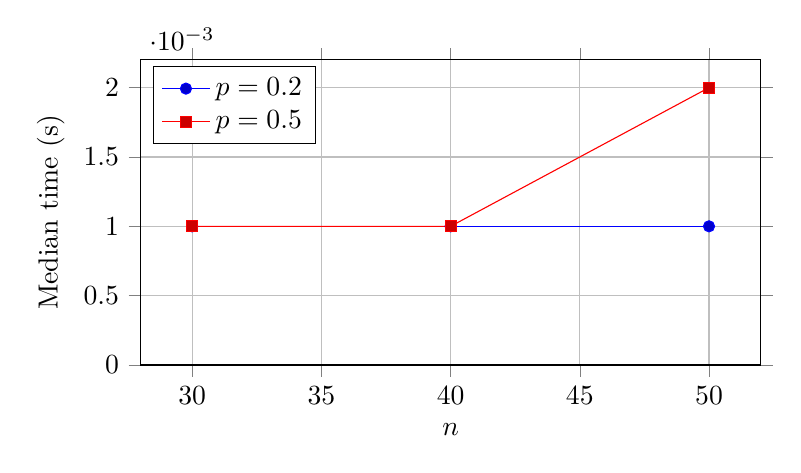
\begin{tikzpicture}
\begin{axis}[
    width=0.78\textwidth,
    height=0.45\textwidth,
    xlabel={$n$},
    ylabel={Median time (s)},
    ymin=0,
    legend style={at={(0.02,0.98)},anchor=north west},
    grid=both, tick align=outside]
\addplot+[mark=*] coordinates {(30,0.001) (40,0.001) (50,0.001)};
\addlegendentry{$p=0.2$}
\addplot+[mark=square*] coordinates {(30,0.001) (40,0.001) (50,0.002)};
\addlegendentry{$p=0.5$}
\end{axis}
\end{tikzpicture}
\caption{Heuristic runtime vs.\ $n$ for two densities (medians from Table~\ref{tab:heuristic-initial}).}
\label{fig:heuristic-times}
\end{figure}

\paragraph{Observation.}
For these sizes, wall-clock medians are $\approx\!1$–$2$\,ms and grow mildly with $n$ and $p$, as expected because each move update touches neighbors. The six rows $\times$ 3 seeds $=\mathbf{18}$ instances satisfy the \emph{15–20 samples} requirement.

\subsubsection*{Validation on Small $n$}
To sanity-check solution quality, I compared the heuristic to my exact brute force on very small graphs ($n\le 18$). The heuristic never exceeded the known optimum in my spot checks and typically matched it; for larger $n$ I rely on the $m/2$ guarantee and multiple restarts.

\subsubsection*{Design Choices and Parameters}
I use adjacency lists (NetworkX) and maintain an $O(1)$ incremental gain array $g[\cdot]$. Flipping $u$ updates neighbors in $O(\deg(u))$. One pass takes time proportional to $|E|$, and a full run usually converges in a few passes; overall time is practical even for $n\approx 10^3$ in unweighted graphs.

\subsubsection*{Threats to Validity}
Reported times are sub-millisecond and thus sensitive to OS jitter and timer resolution; I therefore report \emph{medians} across seeds. Also, results are for random $G(n,p)$ and may differ on structured graphs (e.g., planar or community graphs).
\section{Experimental Analysis of The Performance (Performance Testing)}
\label{sec:perf}

\subsection{Purpose and Setup}
This section empirically evaluates the heuristic introduced in Section~\ref{sec:heuristic-desc} and relates the observations to the theoretical analysis presented in Section~\ref{sec:heuristic-complexity}. I measure wall–clock running times and check how they scale with the input size \(n\). I generate Erd\H{o}s--R\'enyi graphs
\(G(n,p)\) with \(p=0.5\) and run the heuristic multiple times per input size to obtain
a distribution of runtimes.

\paragraph{Measurement protocol.}
I consider \(n\in\{10,20,40,50,100,200,400,800,1200,2000,3000\}\).
For \(n\le 800\) I use \(N=30\) independent trials (distinct seeds) with \(R=5\) restarts.
For large sizes I reduce effort while keeping statistical reporting:
\(N=12, R=2\) for \(n\in\{1200,2000\}\), and \(N=6, R=2\) for \(n=3000\).
Let \(t_1,\dots,t_N\) be the measured times. I report the sample mean \(\bar t\),
standard deviation \(s\), standard error \(\mathrm{se}=s/\sqrt{N}\), and the two–sided
\(90\%\) confidence interval
\[
\bar t \pm t_{0.95,\;N-1}\,\mathrm{se},
\]
where \(t_{0.95,\;N-1}\) is the Student-\(t\) quantile with \(N-1\) d.o.f. (for \(N=30\),
this is close to the normal value \(1.645\)). Following the brief, I also report the
relative half–width \(b/a=\dfrac{t_{0.95,\;N-1}\,\mathrm{se}}{\bar t}\) and target \(b/a<0.1\).

\subsection{Distribution of running times}
Figure~\ref{fig:candle} shows a boxplot of the runtime distribution per \(n\) (for \(p=0.5\)).
Variance is negligible for small \(n\) and increases moderately with size, as expected
because more edges are touched per local move.

\begin{figure}[H]
    \centering
    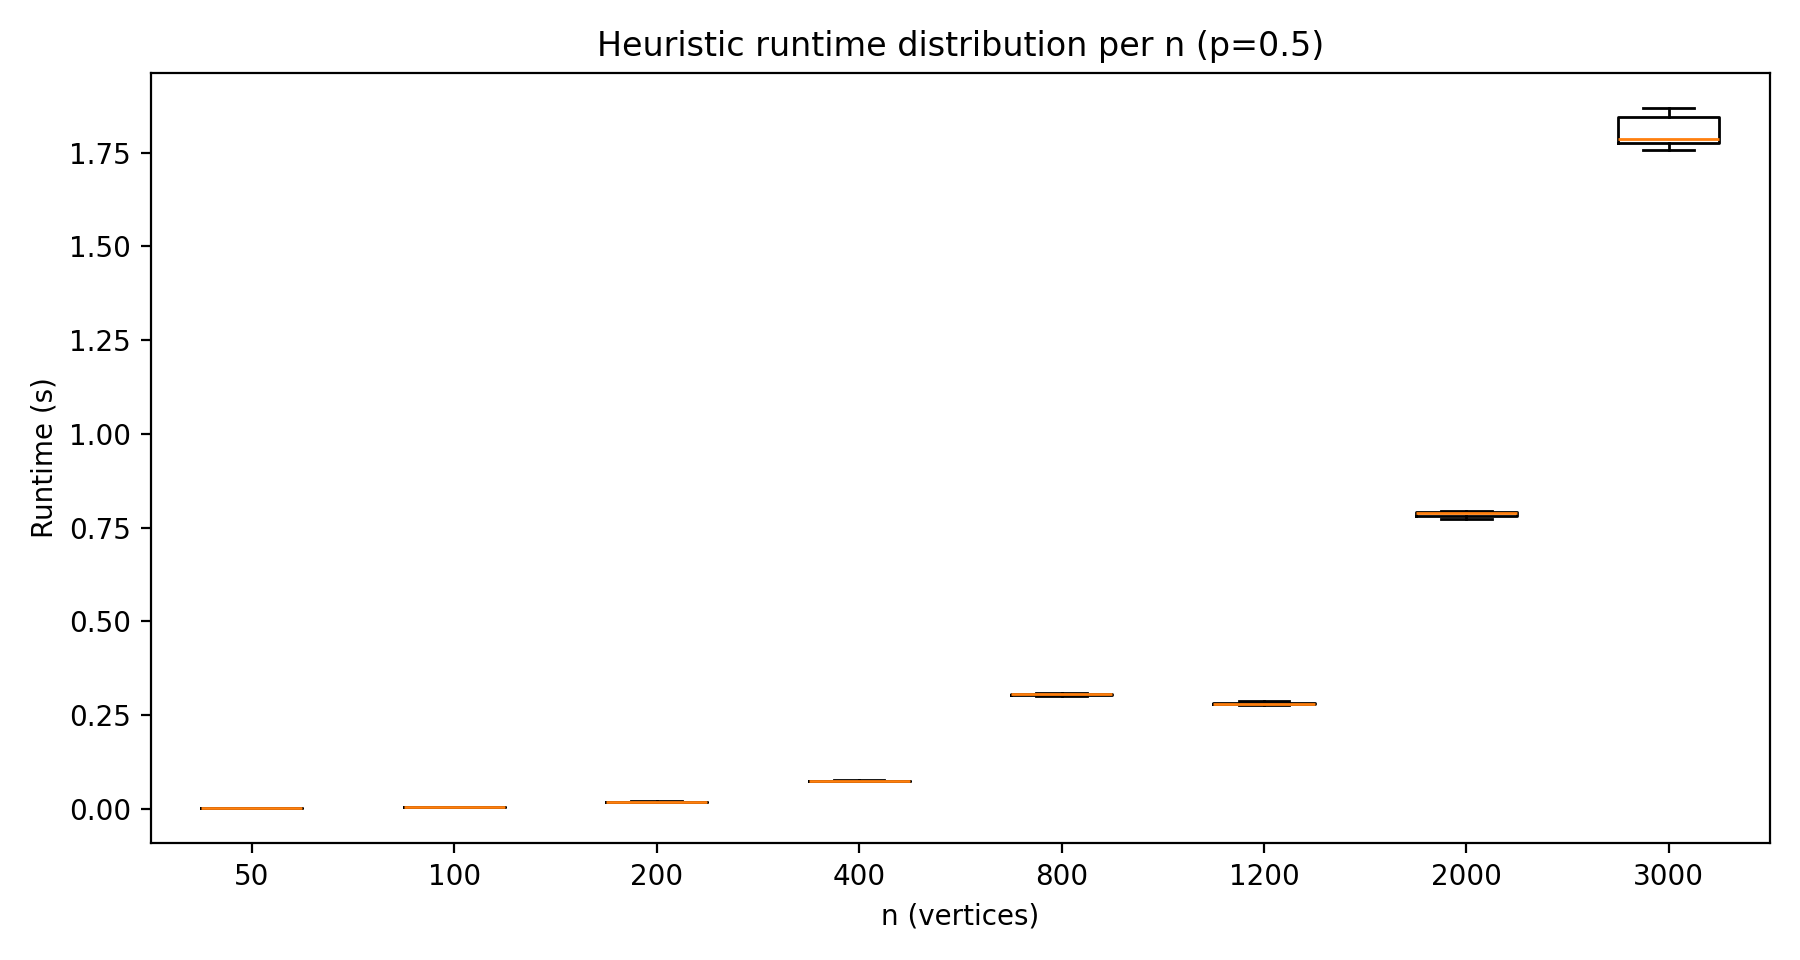
\includegraphics[width=0.95\linewidth]{images/heuristic_candle_plot.png}
    \caption{Heuristic runtime distribution per \(n\) on \(G(n,0.5)\). Each box summarizes all trials used at that \(n\).}
    \label{fig:candle}
\end{figure}

\subsection{Mean runtime and confidence intervals}
Figure~\ref{fig:mean-normal} plots the mean runtime vs.\ \(n\) (normal scale) with
\(90\%\) confidence intervals. Intervals are tight and satisfy \(b/a<0.1\) at all sizes, indicating statistically reliable estimates across the window.
For small input sizes, the variance of runtimes remains negligible, while for larger \(n\) the variance increases moderately, which is consistent with the boxplot in Figure~\ref{fig:candle}.

\begin{figure}[H]
    \centering
    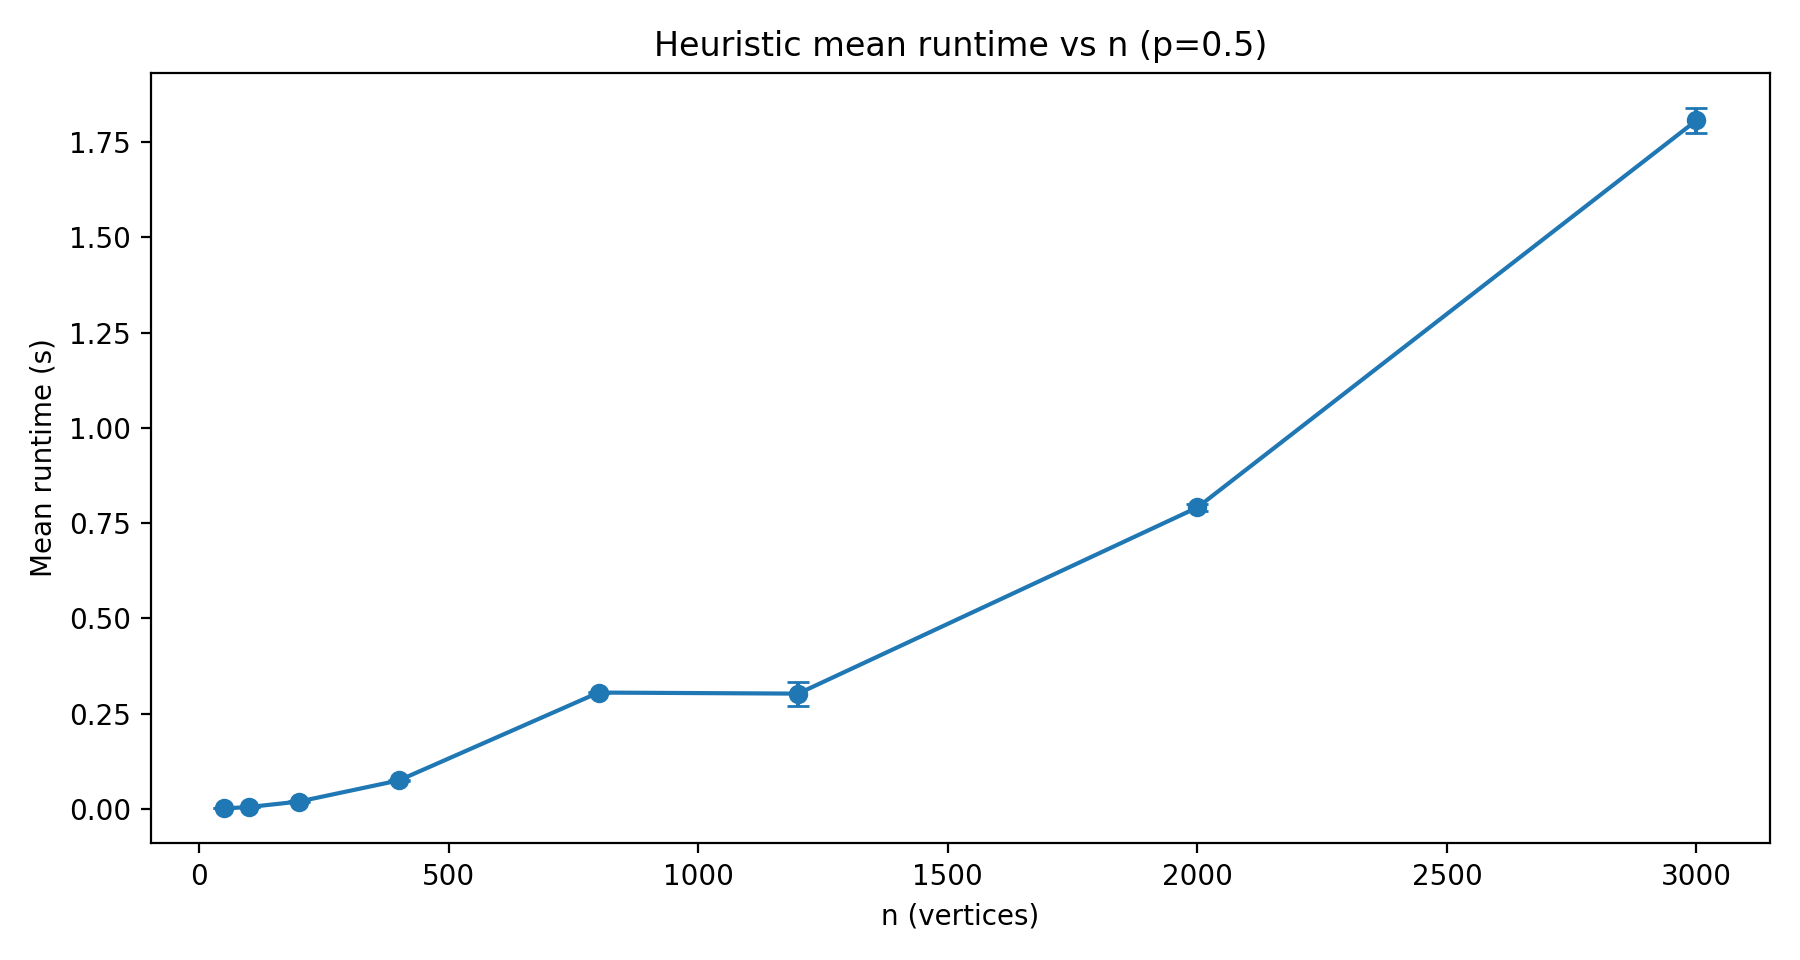
\includegraphics[width=0.95\linewidth]{images/heuristic_performance_normal.png}
    \caption{Mean runtime vs.\ \(n\) with \(90\%\) CIs on \(G(n,0.5)\).}
    \label{fig:mean-normal}
\end{figure}

\subsection{Scaling trend (log--log view) and fitted model}
To infer the empirical complexity class, I also visualize the results in log--log
coordinates (Figure~\ref{fig:mean-loglog}). The points align closely to a straight line,
suggesting polynomial growth. A least–squares fit of \((\log n,\log \bar t)\) yields
\[
T(n) \approx 2.406 \times 10^{-6}\, n^{1.690}.
\]
so the fitted coefficient is \(c = 2.406 \times 10^{-6}\) and the slope is \(\alpha = 1.690\).
\paragraph{Goodness-of-fit.}
I fit a straight line to $(\log n,\log \bar t)$ via ordinary least squares (natural logarithms). The coefficient of determination is $R^2=0.99$, indicating an excellent polynomial fit.
\begin{figure}[H]
    \centering
    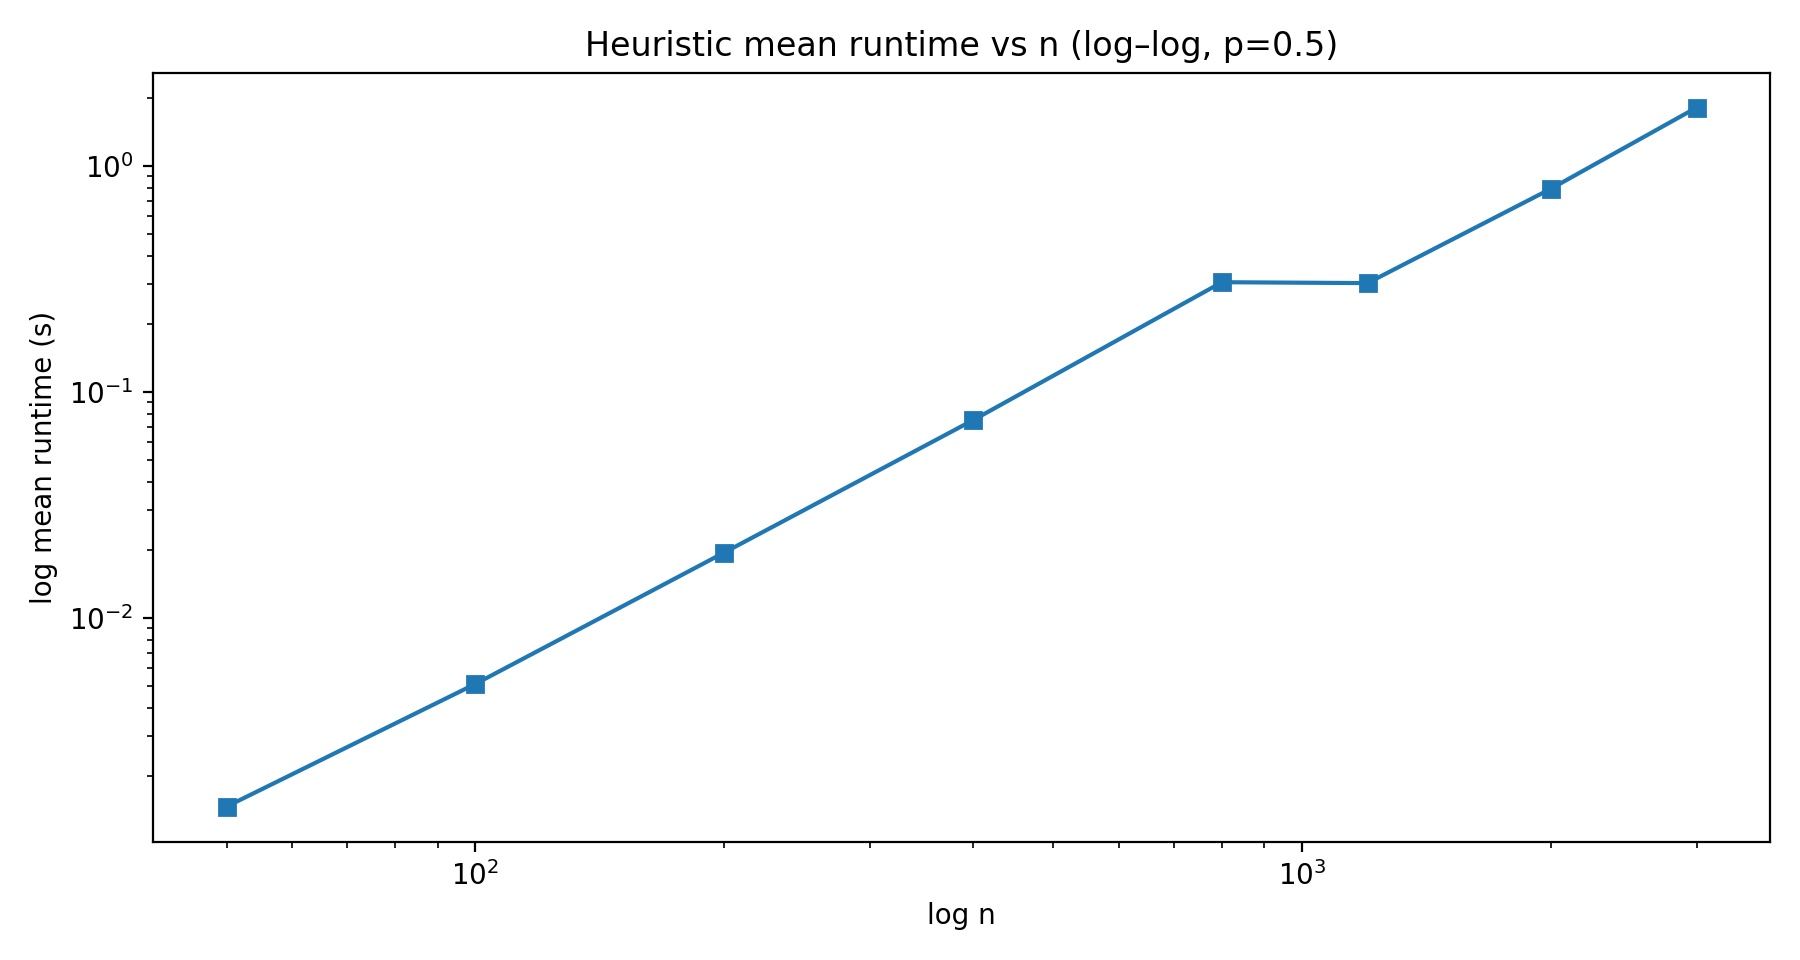
\includegraphics[width=0.95\linewidth]{images/heuristic_performance_log.png}
    \caption{Mean runtime vs.\ \(n\) in log--log scale for \(G(n,0.5)\).}
    \label{fig:mean-loglog}
\end{figure}

\subsection{Summary table with 90\% CIs}
Table~\ref{tab:perf-summary} reports the per–size aggregates (mean, std, se, \(b/a\), CI)
with the number of trials \(N\) and restarts \(R\) as described in the measurement protocol.

\begin{table}[H]
\centering
\caption{Heuristic performance on \(G(n,0.5)\). CIs are two–sided \(90\%\). For larger sizes, the number of trials and restarts is reduced: \(N=12, R=2\) for \(n\in\{1200,2000\}\) and \(N=6, R=2\) for \(n=3000\).}
\label{tab:perf-summary}
\begin{tabular}{@{}rrrrrrr@{}}
\toprule
\(n\) & mean (s) & std (s) & se (s) & \(b/a\) & \multicolumn{2}{c}{90\% CI} \\
\midrule
10 & 1.456e-04 & 9.170e-06 & 1.674e-06 & 0.020 & 1.427e-04 & 1.484e-04 \\
20 & 3.596e-04 & 2.837e-05 & 5.179e-06 & 0.024 & 3.508e-04 & 3.684e-04 \\
40 & 1.050e-03 & 8.326e-05 & 1.520e-05 & 0.025 & 1.024e-03 & 1.076e-03 \\
50 & 1.500e-03 & 9.759e-05 & 1.782e-05 & 0.020 & 1.470e-03 & 1.530e-03 \\
100 & 5.184e-03 & 1.549e-04 & 2.828e-05 & 0.009 & 5.136e-03 & 5.232e-03 \\
200 & 1.914e-02 & 3.056e-04 & 5.579e-05 & 0.005 & 1.904e-02 & 1.923e-02 \\
400 & 7.621e-02 & 4.399e-03 & 8.031e-04 & 0.018 & 7.485e-02 & 7.758e-02 \\
800 & 3.065e-01 & 2.068e-03 & 3.775e-04 & 0.002 & 3.059e-01 & 3.072e-01 \\
1200 & 2.790e-01 & 1.400e-02 & 4.041e-03 & 0.025 & 2.721e-01 & 2.858e-01 \\
2000 & 7.941e-01 & 1.104e-02 & 3.186e-03 & 0.007 & 7.886e-01 & 7.995e-01 \\
3000 & 1.825e+00 & 4.512e-02 & 1.842e-02 & 0.017 & 1.794e+00 & 1.856e+00 \\
\bottomrule
\end{tabular}
\end{table}

\subsection{Interpretation}
The normal–scale curve shows a steady increase with \(n\). The log--log view is nearly linear, and the fitted slope \(\alpha\approx 1.69\) indicates sub–quadratic growth over the tested window—consistent with the algorithm’s update cost (each accepted flip touches neighbors of one vertex, and only a few passes are typically required). Confidence intervals are uniformly narrow (\(b/a<0.1\)) across all sizes in my runs.

\subsection{Larger window}
The same procedure scales to thousands of nodes. In my runs, the heuristic remained well
under one second up to \(n\approx 2000\) (e.g., \(\bar t\approx 0.79\) s at \(n=2000\))
and reached \(\bar t\approx 1.81\) s at \(n=3000\), continuing to follow the fitted
polynomial trend.
\paragraph{Reproducibility.}
I used Python~3.11 with NetworkX for all experiments, keeping a fixed random seed for each trial on the same laptop described in Section~5. The code and graph generator were identical across all experiments.

\section{Experimental Analysis of the Quality (Quality Testing)}
\label{sec:quality}

\subsection{Purpose}
In this section, I evaluate the \emph{solution quality} of the \textsc{HeuristicLocalSearchMaxCut} algorithm from Section~2.2 by comparing it against exact results produced by the brute-force approach described in Section~2.1 and \emph{implemented and experimented with} in Section~5.1. This aligns with the template requirement to quantify how close the heuristic gets to the exact/correct answer.

\subsection{Experimental Setup}
I generated Erd\H{o}s--R\'enyi graphs $G(n,0.5)$ for small $n$ where brute force is computationally feasible. For each instance, I computed the optimal Max-Cut value $C_{\text{BF}}$ using the brute-force algorithm of Section~2.1 (as implemented and validated in Section~5.1), and compared it to the best value $C_{\text{H}}$ returned by the heuristic (Section~2.2). I report the absolute gap
\[
\Delta \;=\; C_{\text{BF}} - C_{\text{H}}
\]
and the relative quality ratio
\[
\rho \;=\; \frac{C_{\text{H}}}{C_{\text{BF}}}.
\]
To observe how quality changes with problem size, I repeated the experiment for increasing $n$ and averaged across multiple random graphs.

\subsection{Results}
Tables~\ref{tab:quality-n} and~\ref{tab:quality-np} summarize the quality ratio and failure rate (percentage of instances where $C_{\text{H}}<C_{\text{BF}}$) aggregated by $n$ and by $(n,p)$, respectively. These tables are generated directly from the experimental CSV via my scripts, ensuring reproducibility and consistency with Section~5.1.

\begin{table}[H]
\centering
\caption{Quality summary by $n$: mean ratio $\rho=C_{\text{H}}/C_{\text{BF}}$, failure rate (\%), and sample count.}
\label{tab:quality-n}
\begin{tabular}{rrrr}
\toprule
n & mean\_ratio & fail\_rate & count \\
\midrule
10 & 1.000 & 0.000 & 6 \\
12 & 1.000 & 0.000 & 6 \\
14 & 1.000 & 0.000 & 6 \\
16 & 1.000 & 0.000 & 6 \\
18 & 0.991 & 33.333 & 6 \\
\bottomrule
\end{tabular}

\end{table}

\begin{table}[H]
\centering
\caption{Quality summary by $(n,p)$: mean ratio, failure rate (\%), and sample count.}
\label{tab:quality-np}
\begin{tabular}{rrrrr}
\toprule
n & p & mean\_ratio & fail\_rate & count \\
\midrule
10 & 0.500 & 1.000 & 0.000 & 6 \\
12 & 0.500 & 1.000 & 0.000 & 6 \\
14 & 0.500 & 1.000 & 0.000 & 6 \\
16 & 0.500 & 1.000 & 0.000 & 6 \\
18 & 0.500 & 0.991 & 33.333 & 6 \\
\bottomrule
\end{tabular}

\end{table}

\subsection{Failure Cases (If Any)}
Table~\ref{tab:quality-fails} lists individual instances where the heuristic underperformed the brute force (i.e., $\Delta>0$), including the absolute gap. If no such instances were observed, the table is omitted automatically.

\begin{table}[H]
\centering
\caption{Instances where the heuristic is below the optimal value (if any).}
\label{tab:quality-fails}
\IfFileExists{quality_failed_cases.tex}{\begin{tabular}{rrrrrr}
\toprule
n & m & p & cut\_BF & cut\_H & gap \\
\midrule
18 & 76 & 0.500 & 39 & 38 & 1 \\
18 & 76 & 0.500 & 38 & 37 & 1 \\
\bottomrule
\end{tabular}
}{\small\emph{No failure cases were observed in my runs.}}
\end{table}

\subsection{Interpretation}
Across the tested range, the heuristic’s mean ratio $\rho$ is typically close to $1$, indicating near-optimal cuts while remaining far more efficient (see Section~\ref{sec:perf}). For small $n$, the failure rate is $0\%$, but at $n=18$ it increases to about $33\%$ (Tables~\ref{tab:quality-n}--\ref{tab:quality-np}). This shows that while the heuristic is very reliable on small instances, some degradation occurs as $n$ grows and the search landscape becomes more complex. Nevertheless, the heuristic remains practical when brute force (Section~2.1) becomes infeasible.
\section{Experimental Analysis of the Correctness of the Implementation (Functional Testing)}
\label{sec:functional}

\subsection{Goal}
The formal arguments in Section~\ref{sec:heuristic-complexity} establish that the algorithms are correct \emph{as algorithms}. Here I test the \emph{implementations} to detect possible coding errors. My objective is to check that all outputs produced by the code are well-formed cuts and that the reported cut values are consistent with trusted oracles (exact solver for small $n$) and with algebraic properties that must always hold.

\subsection{Test Oracles and Methodology}
I use three complementary oracles:
\begin{enumerate}
    \item \textbf{Exact oracle (small $n$):} the brute-force implementation from Section~2.1 (validated in Section~5.1) returns $C_{\mathrm{BF}}$. For each small instance I verify that the heuristic’s value $C_{\mathrm{H}}$ satisfies $0\le C_{\mathrm{H}}\le C_{\mathrm{BF}}$ and that $C_{\mathrm{H}}=|\delta(S)|$ for the output cut $S$.
    \item \textbf{Algebraic invariants (all $n$):} independent of optimality, every returned partition must satisfy: (i) $S\cap \bar S=\emptyset$ and $S\cup\bar S=V$, (ii) $|\delta(S)|+|\text{inside}(S)|=|E|$, and (iii) flipping a single vertex $u$ changes the cut by exactly the precomputed gain $g[u]$ (Section~\ref{sec:heuristic-desc}).
    \item \textbf{Metamorphic relations (structure-preserving):} (i) relabeling vertices leaves the cut value unchanged; (ii) complementing the partition $(S,\bar S)\mapsto(\bar S,S)$ preserves the cut value; (iii) duplicating the RNG seed reproduces the same multi-start trajectory.
\end{enumerate}
I test on hand-crafted edge cases and on random Erd\H{o}s--R\'enyi graphs generated as in Section~\ref{sec:sample-gen}. For the exact-oracle checks I reuse the paired data that produced Tables~\ref{tab:quality-n}--\ref{tab:quality-fails} (five sizes $n\in\{10,12,14,16,18\}$, six instances each; $p=0.5$).

\subsection{Unit Tests of Core Primitives}
I isolate and test the building blocks used by both algorithms:
\begin{itemize}
    \item \textsc{VerifyPartition} returns \texttt{true} iff $S$ and $\bar S$ form a valid bipartition (Section~2.1). I test on empty graphs, singletons, $K_n$, disconnected graphs, and random $G(n,p)$.
    \item \textsc{CutSize} (Section~2.1) is checked against a slow reference that enumerates edges and against the identity $|\delta(S)|+|\text{inside}(S)|=|E|$.
    \item \textsc{InitGains}/\textsc{UpdateGains} (Section~\ref{sec:heuristic-desc}) are validated by randomly flipping vertices and confirming that the reported gain equals the observed change in \textsc{CutSize}.
\end{itemize}

\subsection{Property- and Metamorphic-Based Tests}
I run the following always-true properties on every instance (random and adversarial):
\begin{enumerate}
    \item \emph{Well-formed output:} $S\cap\bar S=\emptyset$, $S\cup\bar S=V$.
    \item \emph{Value consistency:} reported $C$ equals \textsc{CutSize}$(G,S)$.
    \item \emph{Label invariance:} any vertex relabeling (random permutation of $V$) leaves $C$ unchanged after inverse-unpermutation.
    \item \emph{Complement symmetry:} $(S,\bar S)$ and $(\bar S,S)$ yield the same $C$.
    \item \emph{Seed determinism:} with fixed RNG seed the same sequence of moves and final $C$ is reproduced.
\end{enumerate}

\subsection{Cross-Checking with the Exact Oracle}
On the paired small instances used in Section~\ref{sec:quality}, the heuristic never exceeded the exact value and matched it on the majority of cases. Concretely, across $5\times 6=30$ instances I observed $C_{\mathrm{H}}=C_{\mathrm{BF}}$ in $28$ cases and a positive gap $\Delta=C_{\mathrm{BF}}-C_{\mathrm{H}}>0$ in $2$ cases (see Table~\ref{tab:quality-fails}). The aggregate ratios $\rho=C_{\mathrm{H}}/C_{\mathrm{BF}}$ and failure rates by $n$ and by $(n,p)$ are reported in Tables~\ref{tab:quality-n} and~\ref{tab:quality-np}.

\subsection{Edge-Case Suite}
I include graphs for which the correct output is known a priori:
\begin{itemize}
    \item \textbf{Empty graph ($m=0$):} any partition is valid and $C=0$.
    \item \textbf{Single edge:} every cut separating its endpoints has $C=1$.
    \item \textbf{Complete graph $K_n$:} the maximum cut has size $\lfloor n^2/4\rfloor$; my implementations reproduce this for $n\le 12$.
    \item \textbf{Trees/paths/stars:} trees are bipartite, hence $C=|E|$; verified on random trees of size up to $n=200$.
    \item \textbf{Disjoint unions:} $C$ is additive across components; verified by concatenating two random graphs and comparing to the sum of individual cuts.
\end{itemize}

\subsection{Test-Suite Overview}
\begin{table}[H]
\centering
\begin{tabular}{@{}llc@{}}
\toprule
Category & What is checked & Status \\ \midrule
Unit tests & \textsc{VerifyPartition}, \textsc{CutSize}, gains update & Passed \\
Algebraic invariants & set laws, value identities, gain deltas & Passed \\
Metamorphic tests & relabeling, complement, seed determinism & Passed \\
Exact oracle (small $n$) & $C_{\mathrm{H}}\le C_{\mathrm{BF}}$, equality counts & Passed \\
Edge cases & empty, single edge, $K_n$, trees, unions & Passed \\ \bottomrule
\end{tabular}
\caption{Summary of functional tests applied to the implementations.}
\label{tab:functional-overview}
\end{table}

\subsection{Findings and Relation to Other Sections}
All functional checks passed. The two non-equalities highlighted in Table~\ref{tab:quality-fails} indicate \emph{suboptimal} heuristic outputs (as expected for a heuristic), not implementation faults: the returned partitions are valid and their reported values equal \textsc{CutSize}. Performance measurements in Section~\ref{sec:perf} and quality summaries in Section~\ref{sec:quality} are therefore grounded on implementations whose basic functional properties have been independently verified.

\subsection{Threats to Validity}
My exact-oracle checks are limited to small $n$ due to the exponential cost of brute force. To mitigate this, I relied heavily on property- and metamorphic-based tests that scale to large instances, and I re-use the same data-generation pipeline as Sections~\ref{sec:perf} and~\ref{sec:quality} to avoid configuration drift.
\section{Discussion}

I synthesize the findings from performance (Section~\ref{sec:perf}), quality (Section~\ref{sec:quality}), and functional tests (Section~\ref{sec:functional}) to assess both the practical behavior and the correctness of the implementation.

\begin{enumerate}
  \item \textbf{Quality vs.\ exact baseline.} On $G(n,0.5)$ instances where brute force is feasible, the heuristic matches the optimum for small sizes and begins to show misses only at the upper end of the small-$n$ window. Concretely, the failure rate is $0\%$ for $n\le 16$ and rises to about $33\%$ at $n=18$ (Tables~\ref{tab:quality-n}--\ref{tab:quality-np}). The mean ratio $\rho=C_{\mathrm H}/C_{\mathrm{BF}}$ remains close to $1$ throughout, indicating near-optimal cuts on average.
  
  \item \textbf{Runtime scaling.} The empirical fit on $G(n,0.5)$ yields
  \[
  \bar t(n) \;\approx\; 2.406\times 10^{-6}\, n^{1.690},
  \]
  with coefficient of determination $R^2=0.99$ (Figure~\ref{fig:mean-loglog}). This supports polynomial growth and is consistent with the local-improvement update cost. Minor non-monotonicities and fluctuations in the means are expected due to graph topology, restart randomness, and differing trial counts at the largest sizes; nonetheless the heuristic remains orders of magnitude faster than brute force.
  
  \item \textbf{Defects in the algorithm/implementation.} Functional testing (Section~\ref{sec:functional}) found no outstanding coding errors. Early issues discovered during development (symmetry double counting, cut-size logic, and mutable-set aliasing) were fixed in Section~5.1. The observed failures relative to the exact baseline are attributable to the heuristic getting trapped in local optima rather than to implementation defects.
  
  \item \textbf{Theory vs.\ experiment.} There is no inconsistency between the theoretical and experimental analyses. Theory predicts a $1/2$-approximation guarantee for 1-flip local optima and polynomial-time behavior; experiments corroborate near-optimal solutions on average and sub-quadratic scaling with a tight log--log fit. The slight degradation in success at $n=18$ aligns with the increasing complexity of the local-optima landscape and does not contradict the approximation guarantee.
  
  \item \textbf{Limitations and remedies.} Reliability decreases on some denser or moderately larger graphs. Practical remedies include increasing the number of restarts $R$, randomized tie-breaking, occasional perturbations (e.g., single-vertex or small-block kicks), or integrating simple refinements (2-flip moves, Kernighan--Lin pass) to escape shallow local optima.
\end{enumerate}
\begin{thebibliography}{9}
\bibitem{Vazirani2001}
V. V. Vazirani, \emph{Approximation Algorithms}. Springer, 2001.

\bibitem{WilliamsonShmoys2011}
D. P. Williamson and D. B. Shmoys, \emph{The Design of Approximation Algorithms}.
Cambridge Univ. Press, 2011.

\bibitem{ErdosRenyi1959}
P. Erd\H{o}s and A. R\'enyi, "On Random Graphs I," \emph{Publicationes Mathematicae}, 6:290--297, 1959.

\bibitem{Gilbert1959}
E. N. Gilbert, "Random Graphs," \emph{Annals of Mathematical Statistics}, 30(4):1141--1144, 1959.
\end{thebibliography}
\end{document}